% !TeX spellcheck = en_GB
\documentclass[10pt]{beamer}
\usetheme{CambridgeUS}
%\usetheme{Boadilla}
\definecolor{myred}{RGB}{163,0,0}
%\usecolortheme[named=blue]{structure}
\usecolortheme{dove}
\usefonttheme[]{professionalfonts}
\usepackage[english]{babel}
\usepackage{amsmath,amsfonts,amssymb}
\usepackage{xcolor}
\usepackage{tikz}
\tikzset{>=latex}
\usepackage{bm}
\usepackage{textcomp}
\usepackage{gensymb}
\usepackage{caption}
\usepackage{verbatim}
\usepackage{paratype}
\usepackage{mathpazo}
\usepackage{listings}
\usepackage{sgamevar}

\newcommand{\bs}{\boldsymbol}

\newcommand{\cc}[1]{\texttt{\textcolor{blue}{#1}}}

\definecolor{ttcolor}{RGB}{0,0,1}%{RGB}{163,0,0}

% Number theorem environments
\setbeamertemplate{theorem}[ams style]
\setbeamertemplate{theorems}[numbered]

% Reset theorem-like environments so that each is numbered separately
\usepackage{etoolbox}
\undef{\definition}
\theoremstyle{definition}
\newtheorem{definition}{\translate{Definition}}

% Change colours for theorem-like environments
\definecolor{mygreen1}{RGB}{0,96,0}
\definecolor{mygreen2}{RGB}{229,239,229}
\setbeamercolor{block title}{fg=white,bg=mygreen1}
\setbeamercolor{block body}{fg=black,bg=mygreen2}

\lstdefinestyle{numbers}{numbers=left, stepnumber=1, numberstyle=\tiny, numbersep=10pt}
\lstdefinestyle{MyFrame}{backgroundcolor=\color{yellow},frame=shadowbox}

\hypersetup{colorlinks, urlcolor=blue, linkcolor = myred}

\title{R408: Microeconomic Modelling}
\subtitle{Topic XX: \textcolor{myred}{Introduction to Game Theory}}
\author{Andrey Vassilev}

\date{} 

\AtBeginSection{\frame{\usebeamerfont{section title}\centering\insertsection}}

\begin{document}
\maketitle

\begin{frame}[fragile]
\frametitle{Lecture Contents}
\tableofcontents
\end{frame} 

%%%%%%%%%%%%%%%%%%%%%%%%%%%%%
\section{Fundamental concepts of game theory}
%%%%%%%%%%%%%%%%%%%%%%%%%%%%%


\begin{frame}[fragile]
\frametitle{What is a game?}
\framesubtitle{}
\begin{quote}
Drivers manoeuvring in heavy traffic are playing a driving game.
Bargain-hunters bidding on eBay are playing an auctioning game.
A firm and a union negotiating next year's wage are playing a
bargaining game. When opposing candidates choose their
platform in an election, they are playing a political game. The
owner of a grocery store deciding today's price for corn flakes is
playing an economic game. In brief, a game is being played
whenever human beings interact.

\begin{flushright}
-- Ken Binmore, ``Game Theory: A Very Short Introduction'', 2007
\end{flushright}
\end{quote}
\end{frame}



\begin{frame}[fragile]
\frametitle{What is a game?}
\framesubtitle{}
\begin{itemize}\itemsep1em
\item You are already familiar with the idea that rational economic agents will pursue well-defined objectives under certain constraints.
\item This is typically formalized as an optimization problem of some sort (e.g. a static constrained optimization problem or an optimal control problem).
\item In simpler setups, it is assumed that the decision maker controls (optimizes over) certain variables and takes others as completely exogenous. Thus, the outcome will (rather, seems to) depend only on their own decisions.
\item In some situations, however, it is more relevant to take into account that the outcome also depends on the decisions of other persons/entities, each having its own objective.
\item When there are recognized multiperson interactions, there is potential for \emph{strategic interdependence}.
\end{itemize}
\end{frame}



\begin{frame}[fragile]
\frametitle{What is a game?}
\framesubtitle{}
\begin{itemize}\itemsep1em
\item Strategic interdependence implies that we can reason about how other agents will take into account the way everybody plans their actions, and adjust our behaviour accordingly.
\item Everybody else is of course doing the same.
\item \alert{Such situations are called {\color{red}games}.} They are the object of study of \emph{game theory}.
\item Contrast this with the theory of competitive equilibrium, where agents are not directly interested in one another's actions but in certain environment variables (e.g. prices), even though these environment variables are the outcome of everybody's decisions.
\end{itemize}
\end{frame}



\begin{frame}[fragile]\newcounter{examplecount}\setcounter{examplecount}{1}\newcounter{slidenum}\stepcounter{slidenum}
\frametitle{Example \arabic{examplecount}}
\framesubtitle{A first look at a game (\arabic{slidenum})}

\begin{itemize}\itemsep1em
\item Simple games can often be represented in the form of a table.
\item Consider two persons, Player 1 and Player 2, each having at their disposal two possible actions: $\{U,D\} $ for Player 1 and $ \{L,R\} $ for Player 2.
\item They choose simultaneously and independently an action, knowing that the outcome will be determined by the combination of their choices.
\item The outcome takes the form of monetary payoffs to each player and is summarized in the table shown on the next slide.
\end{itemize}
\end{frame}



\begin{frame}[fragile]\stepcounter{slidenum}
\frametitle{Example \arabic{examplecount}}
\framesubtitle{A first look at a game (\arabic{slidenum})}

\begin{center}
\begin{game}{2}{2}[\color{red}Player~1][\color{blue}Player~2]
 \> {\color{blue}$ L $} \> {\color{blue}$ R $}\\
{\color{red} $ U $} \>  $ {\color{red}5},{\color{blue}6} $  \> $ {\color{red}0},{\color{blue}9} $\\
{\color{red} $ D $} \> $ {\color{red}10},{\color{blue}1} $ \> $ {\color{red}3},{\color{blue}2} $
\end{game}
\end{center}\bigskip

Here is a preview of some of the considerations arising in game theoretic situations:
\begin{itemize}\itemsep1em
\item Suppose that Player 1 played $ U $ and Player 2 played $ L $. Will Player 1 regret her choice after the outcome has been revealed? Would she change her mind if given the chance to amend her choice?
\item How about Player 2?
\item What if Player 1 chooses $ U $ and Player 2 chooses $ R $? 
\end{itemize}
\end{frame}



\begin{frame}[fragile]\setcounter{slidenum}{1}
\frametitle{Basic elements of a game (\arabic{slidenum})}
\framesubtitle{}
\begin{itemize}\itemsep1em
\item The above example illustrates the main elements of a game theoretic situation.
\item The entities participating in the game are called the \emph{players}. These can be persons, firms, the government or even nature. In our applications there will be a finite number of players, though sometimes an infinity of players provides a useful abstraction.
\item Each player has at their disposal different \emph{actions}. The actions available will in general depend on the particular situation in the game.
\item A game must have well-specified \emph{rules}. These include e.g. who gets to play at a given stage, what they know, what actions are available to them, when the game should stop, what the outcome for each player will be.
\end{itemize}
\end{frame}



\begin{frame}[fragile]\stepcounter{slidenum}
\frametitle{Basic elements of a game (\arabic{slidenum})}
\framesubtitle{}
\begin{itemize}\itemsep1em
\item The outcomes for the players may be associated with utilities, monetary rewards or, in some cases, costs/expenses. Outcomes are commonly referred to as \emph{payoffs}.
\item Payoffs must obviously be ordered, i.e. the players must have preferences over them. The examples of payoffs given suggest the ordering: 
	\begin{itemize}\itemsep1em
	\item maximize the monetary reward
	\item minimize costs
	\end{itemize}
\item It is somewhat more typical for payoffs to be specified as rewards or utilities. 
\end{itemize}
\end{frame}



\begin{frame}[fragile]
\frametitle{Cooperative and non-cooperative games}
\begin{itemize}\itemsep1em
\item In some games the basic decision-making entity is the individual player. This is the relevant choice when it is assumed that players are independent actors always acting at their own will.
\item In other cases the basic decision-making entity is a group of players, acting as one. This is relevant when prior to the start of the game players can make binding agreements that guarantee the group will act as one entity.
\item The first situation is the subject of \emph{non-cooperative game theory}. The second setup is studied by \emph{cooperative game theory}.
\item We shall study exclusively non-cooperative games, reflecting the thrust of most research done in game theory over the past few decades.
\end{itemize}
\end{frame}



\begin{frame}[fragile]\setcounter{slidenum}{1}
\frametitle{Strategies (\arabic{slidenum})}
\framesubtitle{}
\begin{itemize}\itemsep1em
\item It is often more convenient to study the behaviour of players not in terms of specific actions but in terms of overall plans of behaviour.
\item Such a plan must prescribe what a player should do in every imaginable situation that may arise in the course of a game. A plan like this is called a \emph{strategy}.
\item A strategy can be imagined as a sort of a rulebook: if $ A $ happens, do $ X $; if $ B $ happens, do $ Y $.
\item Sometimes strategies are compared to the aircraft flight manuals used by pilots to apply emergency operating procedures.
\end{itemize}
\end{frame}



\stepcounter{slidenum}
\begin{frame}[fragile]
\frametitle{Strategies (\arabic{slidenum})}
\framesubtitle{}
\begin{itemize}\itemsep1em
\item Strategies can be associated with random choice.
\item One possibility is to choose between overall plans of action randomly. This is similar to choosing at random one of several possible rulebooks and then sticking to its instructions.
\item This is known as a \emph{mixed strategy}.\pause
\item Another possibility is to randomize \emph{within} the rulebook, as if tossing a coin or casting a die to decide what to do in particular situations arising in the course of the game.
\item This is known as a \emph{behaviour strategy}.\pause
\item We shall deal only with mixed strategies in this lecture. As a consolation, under appropriate information assumptions (perfect recall) mixed strategies and behaviour strategies are in a sense equivalent.
\end{itemize}
\end{frame}



\setcounter{slidenum}{1}
\begin{frame}[fragile]
\frametitle{Game representations (\arabic{slidenum})}
\framesubtitle{}
\begin{itemize}\itemsep1em
\item It should be evident from the previous slides that a game can be a complex structure:
	\begin{itemize}\itemsep1em
	\item It can run over time, going through different stages.
	\item Various players can take turns to make choices or act simultaneously.
	\item The actions available to each player can vary in the course of the game.
	\item Players can have different information at different stages.
	\item \ldots
	\end{itemize}
\item If we want to take this complexity on board, then one way to represent a fairly broad class of games is by using special tree-like structures (a specific type of graph).
\item This is known as the \emph{extensive form} of a game.
\end{itemize}
\end{frame}



\begin{frame}[fragile]\stepcounter{slidenum}
\frametitle{Game representations (\arabic{slidenum})}
\begin{itemize}\itemsep1em
\item The players making a decision are represented as the nodes (vertices) of the game tree.
\item The actions available to a player are represented as the edges emanating from a node.
\item Terminal nodes represent the outcomes of the game and are associated with the payoffs for the players.
\end{itemize}
\end{frame}



\begin{frame}[fragile]\stepcounter{slidenum}\stepcounter{examplecount}
\frametitle{Game representations (\arabic{slidenum})}
\framesubtitle{Example \arabic{examplecount}: Sequential version of the Matching Pennies game in extensive form}
\begin{center}
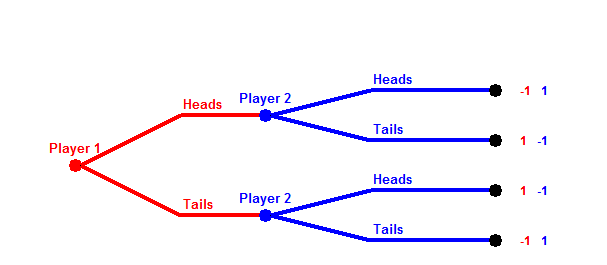
\includegraphics[width=0.8\linewidth]{Sequential_Matching_Pennies}
\end{center}

\begin{itemize}{\small
\item Player 1 puts down a coin heads up or tails up.
\item Player 2 observes this move and also puts down a coin heads up or tails up.
\item If the faces of the two coins match, then Player 2 wins. If they are different, Player 1 wins. (Obviously skewed in favour of Player 2.)}
\end{itemize}
\end{frame}



\begin{frame}[fragile]\stepcounter{slidenum}
\frametitle{Game representations (\arabic{slidenum})}
\begin{itemize}\itemsep1em
\item In certain cases players move simultaneously and neither can observe the others' decisions prior to their own action.
\item In other cases players do not have enough information about the actions taken by others, even though these actions may have already occurred.
\item The above situations are formalized through the concept of an \emph{information set} of a player.
\item Nodes belonging to the same information set are indistinguishable from the point of view of the respective player.
\item To be truly indistinguishable, nodes have to satisfy additional requirements. In particular, the choices available must be the same at all nodes within the same information set and players should not forget what they once knew.
\end{itemize}
\end{frame}



\begin{frame}[fragile]\stepcounter{slidenum}\stepcounter{examplecount}
\frametitle{Game representations (\arabic{slidenum})}
\framesubtitle{Example \arabic{examplecount}: Standard version of the Matching Pennies game in extensive form}
\begin{center}
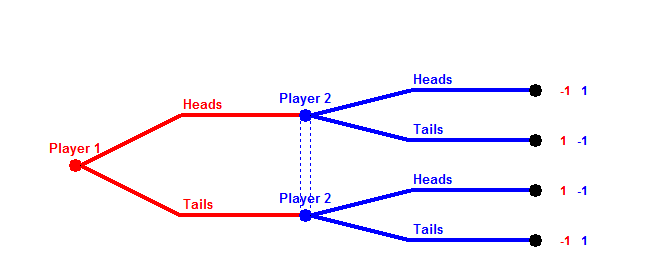
\includegraphics[width=0.8\linewidth]{Standard_Matching_Pennies}
\end{center}

\begin{itemize}{\small
\item Both players put down a coin simultaneously. Or, equivalently, Player 1 puts down his coin first but his choice cannot be observed by Player 2.
\item If the faces of the two coins match, Player 2 wins. If they are different, Player 1 wins.
\item In any case Player 2 does not know Player 1's choice, thus the two blue nodes are in the same information set.
}
\end{itemize}
\end{frame}



\begin{frame}[fragile]\stepcounter{slidenum}
\frametitle{Game representations (\arabic{slidenum})}
\begin{itemize}\itemsep1em
\item Sometimes we are not interested in the details of the sequencing of events in a game but in comparing overall plans of action.
\item Thus, we can study the different strategies available to players without focusing on the specific prescriptions given by a particular strategy.
\item This approach, if deemed acceptable, can help reduce the complexity of the analysis and lead to simpler game representations. However, it also means that once a player has chosen a plan, she will not be allowed to reconsider and deviate from it in the course of the game.
\item A game represented in terms of the strategies available to players is said to be in \emph{strategic form} (or in \emph{normal form}).
\item In simpler cases this leads to a convenient representation of the game in tabular (matrix) form.
\end{itemize}
\end{frame}



\begin{frame}[fragile]\stepcounter{slidenum}\stepcounter{examplecount}
\frametitle{Game representations (\arabic{slidenum})}
\framesubtitle{Example \arabic{examplecount}: Standard version of the Matching Pennies game in strategic form}
\begin{center}
\begin{game}{2}{2}[Player~1][Player~2]
 \> Heads \> Tails \\
Heads \> $ -1,1 $ \> $ 1,-1 $ \\
Tails \> $ 1,-1 $ \> $ -1,1 $
\end{game}
\end{center}\bigskip

\begin{itemize}{\small
\item In this particular case strategies coincide with actions.
}
\end{itemize}
\end{frame}



\begin{frame}[fragile]\stepcounter{slidenum}\stepcounter{examplecount}
\frametitle{Game representations (\arabic{slidenum})}
\framesubtitle{Example \arabic{examplecount}: Sequential version of the Matching Pennies game in strategic form}
\begin{center}
\begin{game}{2}{4}[Player~1][Player~2]
 \> S1 \> S2 \> S3 \> S4 \\
H \> $ -1,1 $ \> $ -1,1 $ \> $ 1,-1 $ \> $ 1,-1 $\\
T \> $ 1,-1 $ \> $ -1,1 $ \> $ 1,-1 $ \> $ -1,1 $
\end{game}
\end{center}\bigskip

\begin{itemize}{\small
\item Description of Player 2's strategies:
	\begin{itemize}
		\item S1 = Play H if Player 1 plays H; play H if Player 1 plays T.
		\item S2 = Play H if Player 1 plays H; play T if Player 1 plays T.
		\item S3 = Play T if Player 1 plays H; play H if Player 1 plays T.
		\item S4 = Play T if Player 1 plays H; play T if Player 1 plays T.
	\end{itemize}
\item Notice how each strategy constitutes a complete contingent plan.
}
\end{itemize}
\end{frame}



\begin{frame}[fragile]\setcounter{slidenum}{1}
\frametitle{Information and knowledge assumptions (\arabic{slidenum})}
\framesubtitle{Perfect vs imperfect information}
\begin{itemize}\itemsep1em
\item If all players always know exactly where they are on the game tree, the game is one of \emph{perfect information}.
\item Formally, this means that all information sets contain exactly one node.
\item Some implications of perfect information are:
	\begin{itemize}\itemsep1em
		\item Players know exactly the entire history of the game, including previous choices made by others and the outcomes of random events.
		\item Simultaneous moves are incompatible with perfect information.
	\end{itemize}
\item As an example, the sequential version of Matching Pennies is a game of perfect information, while the standard version is not.
\end{itemize}
\end{frame}



\begin{frame}[fragile]\stepcounter{slidenum}
\frametitle{Information and knowledge assumptions (\arabic{slidenum})}
\framesubtitle{Complete vs incomplete information}
\begin{itemize}\itemsep1em
\item As a first approximation, it is convenient to assume that the players are well-informed about one another. This includes the assumption that they know their payoffs.
\item However, it is also reasonable to consider situations in which players do not fully know some of the characteristics of the other parties.
\item Such games are called games of \emph{incomplete information}.
\item This stands in contrast to a game of \emph{complete information}, where players are fully informed about the characteristics of others.
\item As an example, decisions to enter a new market can be modelled as a game of incomplete information: the new entrant doesn't know the cost structure of firms that are already operating there.
\end{itemize}
\end{frame}



\begin{frame}[fragile]\stepcounter{slidenum}
\frametitle{Information and knowledge assumptions (\arabic{slidenum})}
\framesubtitle{Perfect vs imperfect recall}
\begin{itemize}\itemsep1em
\item If a player does not forget any information that he knew in the past (e.g. his own moves, others' moves), then the player is said to have perfect recall.
\item Perfect recall is a natural assumption that is often employed in economic applications of game theory, since a rational agent should not be expected to lose or forget information over time.
\item However, it is possible to introduce imperfect recall in a game as a result of using a particular modelling approach. For instance, modelling a team of card players as a single player can lead to imperfect recall.
\end{itemize}
\end{frame}

%%%%%%%%%%%%%%%%%%%%%%%%%%%%%
\section{Games in strategic form}
%%%%%%%%%%%%%%%%%%%%%%%%%%%%%

\begin{frame}[fragile]
\frametitle{General formulation of games in strategic form}
\framesubtitle{}
\begin{itemize}\itemsep1em
\item Even though games in strategic form are often presented in tabular form (as we have already seen), this is not the most general form.
\item A strategic-form game is defined by the following elements:
	\begin{itemize}\itemsep1em
	\item The set of players $ N = \{1,2,\ldots,n\} $.
	\item The set $ S_i $ of strategies available to player $ i\in N $.
	
	The set of all possible strategy vectors is denoted $ S = S_1 \times S_2 \times \cdots \times S_n $. An element of $ S $ is sometimes called a \emph{strategy profile}.
	\item A function $ u_i : S \rightarrow \mathbb{R} $ which gives the payoff to player $ i \in N$ associated with a vector of strategies $ s \in S $.
	\end{itemize}
\item Note that this definition does not require the sets of strategies $ S_i $ to be finite. 
\item \emph{Finite games}, defined by the fact that the players' strategy sets are finite, are a special case that is representable in tabular form.
\end{itemize}
\end{frame}




\setcounter{slidenum}{1}
\begin{frame}[fragile]
\frametitle{Dominance (\arabic{slidenum})}
\begin{itemize}\itemsep1em
\item We now move forward in trying to develop some components of a theory of reasonable behaviour in games.
\item The first idea we consider is that if, for every possible situation, some strategy leaves a player better off than another strategy, then the second strategy should not be used.
\item Formally, the second strategy is a \emph{dominated strategy}.
\end{itemize}
\end{frame}



\stepcounter{examplecount}
\begin{frame}[fragile]\stepcounter{slidenum}
\frametitle{Dominance (\arabic{slidenum})}
\framesubtitle{Example \arabic{examplecount}}
To  illustrate the idea of a dominated strategy, take the following game:
\begin{center}
\begin{game}{2}{3}[Player~1][Player~2]
 \> $ L $ \> $ M $ \> $ R $ \\
$ T $ \> $ 5,5 $ \> $ 1,1 $ \> $ 1,0 $ \\
$ B $ \> $ 1,1 $ \> $ 5,5 $ \> $ 5,0 $
\end{game}
\end{center}

\begin{itemize}\itemsep1em
\item Whatever Player 1 does, strategy $ M $ ensures that Player 2 will have a higher payoff compared to strategy $ R $.
\item Strategy $ R $ is called a \emph{strictly dominated strategy}.
\item It is possible to have strategies that are \emph{weakly dominated}, i.e. they do worse compared to another strategy for some of the opponents' actions and do equally well for others.
\end{itemize}
\end{frame}



\setcounter{slidenum}{1}
\begin{frame}[fragile]
\frametitle{A first look at Gambit (\arabic{slidenum})}
\begin{itemize}\itemsep1em
\item Gambit (\url{http://www.gambit-project.org/}) is a software that solves certain classes of game theory problems.
\item It has a GUI-based version, which we shall use here, as well as the possibility to access its functionality programmatically via a set of command-line tools or a Python interface.
\item It can work with games in strategic and in extensive form.
\item One of its functionalities is related to finding dominated strategies.
\end{itemize}
\end{frame}



\begin{frame}[fragile]\stepcounter{slidenum}
\frametitle{A first look at Gambit (\arabic{slidenum})}
\framesubtitle{Guided exercise}
\begin{itemize}\itemsep1em
\item Input the game from Example \arabic{examplecount} in Gambit. We restate it here for convenience:
\begin{center}
\begin{game}{2}{3}[Player~1][Player~2]
 \> $ L $ \> $ M $ \> $ R $ \\
$ T $ \> $ 5,5 $ \> $ 1,1 $ \> $ 1,0 $ \\
$ B $ \> $ 1,1 $ \> $ 5,5 $ \> $ 5,0 $
\end{game}
\end{center}
\item What are the results when you study dominance via the Gambit interface?
\end{itemize}
\end{frame}



\setcounter{slidenum}{1}
\begin{frame}[fragile]
\frametitle{Iterated elimination of dominated strategies (\arabic{slidenum})}
\begin{itemize}\itemsep1em
\item The existence of a dominated strategy effectively reduces the choices of the respective player.
\item If players behave rationally they should not play a dominated strategy. Moreover, all players should know that everybody else is also rational, and all should know that all know ... (common knowledge).
\item If the above is true, we can proceed to eliminate dominated strategies, arriving at a reduced game.
\item Such a reduced game may in turn be analysed to further eliminate newly emerged dominated strategies, arriving at a still smaller game.
\item This process can terminate at some intermediate stage or it can end when there is only one strategy left per player.
\item In the latter case the resulting strategy profile can be regarded as a solution to the game.
\end{itemize}
\end{frame}


\stepcounter{examplecount}
\begin{frame}[fragile]\stepcounter{slidenum}
\frametitle{Iterated elimination of dominated strategies (\arabic{slidenum})}
\framesubtitle{Example \arabic{examplecount}}
Take a look at the game shown below:
\begin{center}
\begin{game}{3}{3}[Player~1][Player~2]
 \> $ L $ \> $ M $ \> $ R $ \\
$ U $ \> $ 4,3 $ \> $ 5,1 $ \> $ 6,2 $ \\
$ M $ \> $ 2,1 $ \> $ 8,4 $ \> $ 3,6 $ \\
$ D $ \> $ 3,0 $ \> $ 9,6 $ \> $ 2,8 $
\end{game}
\end{center}\bigskip

\begin{itemize}\itemsep1em
\item In this game, strategy $ M $ is strictly dominated by strategy R for Player 2.
\item Therefore, Player 2 should not play strategy $ M $, which results in a new, ``smaller'' game.
\end{itemize}
\end{frame}



\begin{frame}[fragile]\stepcounter{slidenum}
\frametitle{Iterated elimination of dominated strategies (\arabic{slidenum})}
\framesubtitle{Example \arabic{examplecount}}
The reduced game now is:
\begin{center}
\begin{game}{3}{2}[Player~1][Player~2]
 \> $ L $ \>  $ R $ \\
$ U $ \> $ 4,3 $ \>  $ 6,2 $ \\
$ M $ \> $ 2,1 $ \>  $ 3,6 $ \\
$ D $ \> $ 3,0 $ \>  $ 2,8 $
\end{game}
\end{center}\bigskip

\begin{itemize}\itemsep1em
\item In this game strategy $ U $ will provide better outcomes for Player 1 than strategies $ M $ or $ D $.
\item Since strategies $ M $ and $ D $ are now strictly dominated (note that they weren't in the original game), they can be eliminated from consideration, resulting in an even smaller game. 
\end{itemize}
\end{frame}



\begin{frame}[fragile]\stepcounter{slidenum}
\frametitle{Iterated elimination of dominated strategies (\arabic{slidenum})}
\framesubtitle{Example \arabic{examplecount}}
The game now takes the following form:
\begin{center}
\begin{game}{1}{2}[Player~1][Player~2]
 \> $ L $ \>  $ R $ \\
$ U $ \> $ 4,3 $ \>  $ 6,2 $ \\
\end{game}
\end{center}\bigskip

\begin{itemize}\itemsep1em
\item In this game Player 2 is better off playing $ L $, i.e. strategy $ R $ is now dominated.
\item Thus, we are left with the strategy profile $ (U,L) $, yielding payoffs $ 4 $ and $ 3 $ to Player 1 and Player 2, respectively.
\end{itemize}
\end{frame}


\begin{frame}[fragile]\stepcounter{slidenum}
\frametitle{Iterated elimination of dominated strategies (\arabic{slidenum})}
\begin{itemize}\itemsep1em
\item As our first example of a dominated strategy shows, a game is not always guaranteed to have a solution in terms of iterated elimination of dominated strategies.
\item However, in the special case where each player has a \emph{strictly dominant} strategy, i.e. one dominating all the other strategies for that player, the game will have a solution in strictly dominant strategies.
\item Again, the assumption of common knowledge is crucial for the elimination procedure to work.
\end{itemize}
\end{frame}


\begin{frame}[fragile]
\frametitle{Exercise on iterated elimination of dominated strategies}
Consider the following game:
\begin{center}
\begin{game}{3}{3}[Player~1][Player~2]
 \> $ L $ \> $ M $ \> $ R $ \\
$ T $ \> $ 1,0 $ \> $ 1,2 $ \> $ 0,1 $ \\
$ B $ \> $ 0,3 $ \> $ 0,1 $ \> $ 2,0 $
\end{game}
\end{center}\bigskip

\begin{itemize}\itemsep1em
\item Input the game in Gambit.
\item Study what happens when you repeatedly eliminate dominated strategies. Can you explain the outcomes?
\end{itemize}

\end{frame}




\begin{frame}[fragile]
\frametitle{Nash equilibria}
\framesubtitle{Motivation}
\begin{itemize}\itemsep1em
\item Iterated elimination of dominated strategies provides one possibility of predicting the outcome of a game. Unfortunately, it is not applicable to many games.
\item Another approach to the analysis of a game is to look for some sort of stable outcome.
\item One definition of ``stability'' of an outcome is based on the idea that in a stable outcome no-one should have incentives to unilaterally deviate from his chosen strategy if given that choice.
\item This idea forms the basis of the so-called \emph{Nash equilibrium}.
\end{itemize}
\end{frame}



\begin{frame}[fragile]
\frametitle{Nash equilibria}
\framesubtitle{Definition}
We introduce the following notation: if $ s_i $ is the strategy of player $ i $ in a strategy vector $ s $, then the strategies of all the other players in $ s $ will be denoted by $ s_{-i} $.\bigskip

\begin{definition}[Nash equilibrium]\label{def:NashEq}
A strategy vector $ s^* = (s_1^*,\ldots,s_n^*) $ is a \emph{Nash equilibrium} if for each player $ i \in N $ and each strategy $ s_i \in S_i $ the following is satisfied:
\begin{equation}
u_i(s^*)\geq u_i(s_i,s^*_{-i}).
\label{eq:NE}
\end{equation}

The payoff vector $ u(s^*) = (u_1(s*),\ldots,u_n(s^*) $ is the equilibrium payoff corresponding to Nash equilibrium $ s^* $.
\end{definition}
\end{frame}



\begin{frame}[fragile]
\frametitle{Nash equilibria}
\framesubtitle{Existence and uniqueness of Nash equilibria}
\begin{itemize}\itemsep1em
\item Nash equilibria need not exist for an arbitrary game.
\item Their existence is guaranteed under special technical assumptions. We shall not go into the details of the existence results but shall confine ourselves to cases where Nash equilibria exist.
\item It is useful to know from the start that we may need to resort to the notion of a mixed strategy (mentioned earlier) if we want to ensure existence.
\item In cases where there is a Nash equilibrium, it need not be unique.
\end{itemize}
\end{frame}



\setcounter{slidenum}{1}
\begin{frame}[fragile]
\frametitle{Best replies and Nash equilibria (\arabic{slidenum})}
\framesubtitle{}
\begin{itemize}\itemsep1em
\item An equivalent way of defining a Nash equilibrium is through the concept of a \emph{best reply}.
\item It is sometimes more convenient to work with best replies since they provide a natural approach to computing Nash equilibria.
\end{itemize}

\begin{definition}[Best reply]\label{def:BR}
Let $ s_{-i} $ be a strategy vector of all the players except player $ i $. Player $ i $'s strategy $ s_i $ is called a \emph{best reply} to $ s_{-i} $ if \begin{equation}
u_i(s_i,s_{-i}) = \max_{t_i \in S_i}u_i(t_i,s_{-i}).
\label{eq:BR}
\end{equation}
\end{definition}
\end{frame}



\begin{frame}[fragile]\stepcounter{slidenum}
\frametitle{Best replies and Nash equilibria (\arabic{slidenum})}
\framesubtitle{}
The following definition of a Nash equilibrium can be shown to be \textbf{equivalent} to Definition \ref{def:NashEq}:\bigskip

\begin{definition}[Nash equilibrium]\label{def:NashEq2}
A strategy vector $ s^* = (s_1^*,\ldots,s_n^*) $ is a \emph{Nash equilibrium} if $ s_i^* $ is a best reply to $ s_{-i}^* $ for every player $ i \in N $.
\end{definition}
\end{frame}



\begin{frame}[fragile]\stepcounter{examplecount}
\frametitle{Example \arabic{examplecount}}
\framesubtitle{An obvious Nash equilibrium}

\begin{center}
\begin{game}{2}{2}[Player~1][Player~2]
 \> $ X $ \> $ Y $ \\
$ A $ \> $ 5,5 $ \> $ 1,1 $ \\
$ B $ \> $ 1,1 $ \> $ 0,0 $
\end{game}
\end{center}\bigskip

\begin{itemize}\itemsep1em
\item It is obvious that $ (A,X) $ is an equilibrium: it yields the highest possible payoffs for both players and there are no incentives to deviate from it.
\item The interests of both players coincide and there is no element of conflict in the game.
\item In that sense this game is trivial.
\item Another way of looking at this game would be to notice that $ (A,X) $ is a solution in strictly dominant strategies for the game.
\end{itemize}
\end{frame}



\begin{frame}[fragile]\stepcounter{examplecount}\setcounter{slidenum}{1}
\frametitle{Example \arabic{examplecount}}
\framesubtitle{Prisoner's Dilemma (\arabic{slidenum})}
\begin{itemize}\itemsep1em
\item Two persons are arrested on suspicion of committing a serious crime. The sentence for this crime is 10 years in prison.
\item However, evidence is insufficient and they can only be sentenced to 1 year in prison for a lesser crime.
\item The suspects are held in separate cells and cannot communicate.
\item The prosecutor offers each of them a deal: if they tell on their friend (defect, strategy $ D $), they will receive immunity as a state witness (i.e. 0 years in prison) and the friend gets the full 10 years.
\end{itemize}
\end{frame}

\begin{frame}[fragile]
\frametitle{Example \arabic{examplecount}}\stepcounter{slidenum}
\framesubtitle{Prisoner's Dilemma (\arabic{slidenum})}
\begin{itemize}\itemsep1em
\item If they cooperate with each other and remain silent (strategy $ C $), they get 1 year in prison each for the small crime.
\item If both suspects defect, they get an intermediate sentence of 6 years in prison, since their confession is counted as mitigating behaviour in court.
\item The prisoners are asked to make their choices on the prosecutor's offer independently and simultaneously. No information is exchanged in the process.
\end{itemize}
\end{frame}

\begin{frame}[fragile]
\frametitle{Example \arabic{examplecount}}\stepcounter{slidenum}
\framesubtitle{Prisoner's Dilemma (\arabic{slidenum})}
\begin{center}
\begin{game}{2}{2}[Player~1][Player~2][The Prisoner's Dilemma: outcomes presented as years in prison.]
 \> $ D $ \> $ C $ \\
$ D $ \> $ 6,6 $ \> $ 0,10 $ \\
$ C $ \> $ 10,0 $ \> $ 1,1 $
\end{game}
\end{center}\bigskip

\begin{itemize}\itemsep1em
\item This game has one Nash equilibrium, $ (D,D) $, with a payoff profile of $ (6,6) $.
\item It is easy to verify that, whatever the choice of the other player, a player who played $ C $ would wish he had played $ D $ instead.
\item Indeed, $ C $ is a dominated strategy in this game.
\end{itemize}
\end{frame}

\begin{frame}[fragile]
\frametitle{Nash equilibria and Pareto optimality}
\framesubtitle{}
\begin{itemize}\itemsep1em
\item The example of the Prisoner's Dilemma shows that a Nash equilibrium need not be Pareto optimal.
\item The outcome $ (6,6) $ is Pareto-dominated by $ (1,1) $, obtainable if both players choose to cooperate.
\item Thus, strategic incentives may lead to a deviation from social optimality.
\item This stands in contrast to the case of competitive equilibrium, which is Pareto optimal by virtue of the First Fundamental Theorem of Welfare Economics.
\end{itemize}
\end{frame}

\begin{frame}[fragile]
\frametitle{The limitations of pure strategies}
\framesubtitle{}
\begin{itemize}\itemsep1em
\item So far we worked only with the elements of the strategy sets $ S_i $ directly, i.e. with pure strategies.
\item Under this approach many interesting games do not have Nash equilibria.
\item The standard version of Matching Pennies provides an illustration:
\begin{center}
\begin{game}{2}{2}[Player~1][Player~2]
 \> Heads \> Tails \\
Heads \> $ -1,1 $ \> $ 1,-1 $ \\
Tails \> $ 1,-1 $ \> $ -1,1 $
\end{game}
\end{center}\bigskip
\item For any pure strategy profile in this game, one of the players will find an alternative strategy yielding a higher payoff.
\end{itemize}
\end{frame}

\setcounter{slidenum}{1}
\begin{frame}[fragile]
\frametitle{Mixed strategies (\arabic{slidenum})}
\framesubtitle{}
\begin{itemize}\itemsep1em
\item One answer to this limitation of pure strategies is to extend the notion of a strategy and consider the set of all distributions over the pure strategies of a player. 
\item These are the \emph{mixed strategies} we mentioned previously.
\item In the case of finite games mixed strategies are relatively simple objects.
\item In this framework a pure strategy can be regarded as a special case of a mixed strategy placing probability $ 1 $ on a particular element.
\item Mixed strategies are also convenient in terms of their interpretation. For example, if we treat a mixed strategy as randomization over pure strategies, then sometimes being unpredictable can provide an additional strategic advantage (think of a poker player who bluffs occasionally).
\item \textbf{Warning:} Mixed strategies can have different interpretations. The direct interpretation as a deliberate randomization choice is only one possibility.
\end{itemize}
\end{frame}


\begin{frame}[fragile]\stepcounter{slidenum}
\frametitle{Mixed strategies (\arabic{slidenum})}
\framesubtitle{}
\begin{definition}
If $ G = (N,\{S_i\}_{i \in N}, \{u_i\}_{i \in N}) $ is a finite strategic-form game, then the set \begin{equation}
\Sigma_i := \left\{\, \sigma_i: S_i \rightarrow [0,1] \mid \sum_{s_i \in S_i}\sigma_i(s_i) = 1  \,\right\}
\label{eq:MixedStrSet}
\end{equation}
is the set of mixed strategies for player $ i $. The set of mixed strategy profiles is $ \Sigma = \Sigma_1 \times \cdots \times \Sigma_n $.
\label{def:MixedStr}
\end{definition}\bigskip

For a finite set $ A $, we can define the set \[ \Delta(A) := \left\{\, p: A \rightarrow [0,1] \mid \sum_{a\in A}p(a) = 1  \,\right\}, \] which is called a \emph{simplex} in $ \mathbb{R}^{|A|} $. Thus, we have $ \Sigma_i = \Delta(S_i) $.
\end{frame}



\begin{frame}[fragile]
\frametitle{The mixed extension of a game}
\framesubtitle{}
\begin{definition}[Mixed extension of $ G $]
Let $ G $ be a finite strategic-form game. The \emph{mixed extension} of $ G $ is the game \begin{equation}
\Gamma := \left(N,\{\Sigma_i\}_{i \in N}, \{U_i\}_{i \in N}\right) ,
\label{eq:MixedExtG}
\end{equation}
where the expected payoff functions $ U_i : \Sigma \rightarrow \mathbb{R} $ are defined as
\begin{equation}
U_i(\sigma) = \mathbb{E}_{\sigma}[u_i(\sigma)] = \sum_{(s_1,\ldots,s_n)\in S}u_i(s_1,\ldots,s_n)\sigma_1(s_1)\sigma_2(s_2)\cdots \sigma_n(s_n).
\label{eq:ExpPayoff}
\end{equation}
\label{def:MixedExtension}
\end{definition}
\end{frame}


\begin{frame}[fragile]
\frametitle{Nash equilibria in mixed strategies}
\framesubtitle{}
\begin{itemize}\itemsep1em
\item The concept of Nash equilibrium can be applied to the mixed extension $ \Gamma $ of a finite strategic-form game $ G $.
\item It can be shown that a Nash equilibrium in mixed strategies always exists for a finite game (i.e. one with a finite number of players, each having a finite pure strategy set $ S_i $).
\end{itemize}
\end{frame}



\begin{frame}[fragile]\stepcounter{examplecount}\setcounter{slidenum}{1}
\frametitle{Example \arabic{examplecount}}
\framesubtitle{A pure coordination game (\arabic{slidenum})}
Consider the following game:
\begin{center}
\begin{game}{2}{2}[Player~1][Player~2]
 \> $ X $ \> $ Y $ \\
$ A $ \> $ 2,2 $ \> $ 0,0 $ \\
$ B $ \> $ 0,0 $ \> $ 2,2 $
\end{game}
\end{center}\bigskip

\begin{itemize}\itemsep1em
\item Such a game is called a coordination game: players can benefit from matching (coordinating) their strategies.
\item One can verify directly that the game has two pure strategy Nash equilibria: $ (A,X) $ and $ (B,Y) $
\item Can we recover them in a mixed strategy framework? Are there any other Nash equilibria in mixed strategies?
\end{itemize}
\end{frame}

\begin{frame}[fragile]\stepcounter{slidenum}
\frametitle{Example \arabic{examplecount}}
\framesubtitle{A pure coordination game (\arabic{slidenum})}
\begin{itemize}\itemsep1em
\item Denote a mixed strategy for player $ i $ by $ (p_1^i,p_2^i) $.
\item The expected payoff to Player 1 from a given mixed strategy profile is
\[ (p^1_1,p^1_2)\begin{pmatrix}
2 & 0\\
0 & 2
\end{pmatrix}\begin{pmatrix}
p^2_1 \\
%{}\\
p^2_2
\end{pmatrix} = (p^1_1,1-p^1_1)\begin{pmatrix}
2 & 0\\
0 & 2
\end{pmatrix}\begin{pmatrix}
p^2_1 \\
%{}\\
1-p^2_1
\end{pmatrix}.\]
\item The expected payoff to Player 2 is actually the same by virtue of the structure of the game.
\item Such a payoff can be written as \[ 2p^1_1p^2_1 + 2 (1-p^1_1)(1-p^2_1) = 2(2p_1^2 -1)p_1^1 + 2(1-p^2_1). \]
\end{itemize}
\end{frame}


\begin{frame}[fragile]\stepcounter{slidenum}
\frametitle{Example \arabic{examplecount}}
\framesubtitle{A pure coordination game (\arabic{slidenum})}
\begin{itemize}\itemsep1em
\item This payoff is maximized for:
	\begin{itemize}\itemsep1em
	\item $ p^1_1 = 0 $ if $ p^2_1 < \frac{1}{2} $,
	\item $ p^1_1 = 1 $ if $ p^2_1 > \frac{1}{2} $,
	\item any $ p^1_1 $ if $ p^2_1 = \frac{1}{2} $.
	\end{itemize} 
\item A symmetric argument is valid for Player 2.
\item Thus, \emph{both} players' expected payoffs are maximized for the mixed strategy profiles $ [(1,0); (1,0)] $ and $ [(0,1); (0,1)] $, i.e. we have recovered the pure strategy equilibria.
\item In addition, the profile $ [(0.5,0.5); (0.5,0.5)] $ turns out to be a Nash equilibrium as well. It is an equilibrium in mixed strategies.
\end{itemize}
\end{frame}



\begin{frame}[fragile]\stepcounter{examplecount}\setcounter{slidenum}{1}
\frametitle{Example \arabic{examplecount}}
\framesubtitle{Battle of the Sexes (\arabic{slidenum})}
\begin{itemize}\itemsep1em
\item A man and a woman have to decide how to spend an evening together.
\item They have two options: going to a football game ($ F $) or going to a concert ($ C $).
\item The man prefers the football game, while the woman prefers the concert.
\item Yet, each would choose to go to the less preferable event with their partner, rather than going to their favourite event alone.
\end{itemize}
\end{frame}


\begin{frame}[fragile]\stepcounter{slidenum}
\frametitle{Example \arabic{examplecount}}
\framesubtitle{Battle of the Sexes (\arabic{slidenum})}
\begin{center}
\begin{game}{2}{2}[Man][Woman]
 \> $ F $ \> $ C $ \\
$ F $ \> $ 2,1 $ \> $ 0,0 $ \\
$ C $ \> $ 0,0 $ \> $ 1,2 $
\end{game}
\end{center}\bigskip

\begin{itemize}\itemsep1em
\item The game has several Nash equilibria.
\item There are two equilibria in pure strategies: $ (F,F) $ and $ (C,C) $.
\item There is also one equilibrium in mixed strategies with probabilities $ (\frac{2}{3},\frac{1}{3}) $ for the man and probabilities $ (\frac{1}{3},\frac{2}{3}) $ for the woman.
\end{itemize}
\end{frame}

\begin{frame}[fragile]
\frametitle{Exercise on the Battle of the Sexes}
\framesubtitle{}
\begin{enumerate}\itemsep1em
\item Input the game in Gambit.
\item Check if there are dominated strategies.
\item Compute all Nash equilibria and verify the claims from the previous slide.
\end{enumerate}
\end{frame}



\begin{frame}[fragile]\stepcounter{examplecount}\setcounter{slidenum}{1}
\frametitle{Example \arabic{examplecount}}
\framesubtitle{Rock-paper-scissors (\arabic{slidenum})}
\begin{itemize}\itemsep1em
\item This example formalizes the well-known hand game of the same name.
\item There are two players.
\item Each player chooses between three actions: \emph{Rock}, \emph{Paper} or \emph{Scissors}. The choices are made simultaneously.
\item The outcomes are determined by the following rules:
	\begin{itemize}\itemsep1em
	\item Identical choices, e.g. (Rock,Rock), result in a tie.
	\item \emph{Rock} wins over \emph{Scissors} (``Rock breaks scissors'')
	\item \emph{Scissors} wins over \emph{Paper} (``Scissors cuts paper'')
	\item \emph{Paper} wins over \emph{Rock} (``Paper wraps rock'')
	\end{itemize}
\item The game is zero-sum: a win for one player is a loss for the other.
\end{itemize}
\end{frame}


\begin{frame}[fragile]\stepcounter{slidenum}
\frametitle{Example \arabic{examplecount}}
\framesubtitle{Rock-paper-scissors (\arabic{slidenum})}
\begin{center}
\begin{game}{3}{3}[Player~1][Player~2]
 \> Rock \> Paper \> Scissors \\
Rock \> $ 0,0 $ \> $ -1,1 $ \> $ 1,-1 $ \\
Paper \> $ 1,-1 $ \> $ 0,0 $ \> $ -1,1 $ \\
Scissors \> $ -1,1 $ \> $ 1,-1 $ \> $ 0,0 $
\end{game}
\end{center}\bigskip

\begin{itemize}\itemsep1em
\item It can be verified immediately that the game has no Nash equilibrium in pure strategies: for any strategy profile either the losing player or both players would like to unilaterally change their choice, if possible.
\item The game has one equilibrium in mixed strategies: $ (\frac{1}{3},\frac{1}{3},\frac{1}{3}) $ for Player 1 and also $ (\frac{1}{3},\frac{1}{3},\frac{1}{3}) $ for Player 2.
\end{itemize}
\end{frame}

\begin{frame}[fragile]
\frametitle{Exercise on Rock-paper-scissors}
\framesubtitle{}
\begin{enumerate}\itemsep1em
\item Input the game in Gambit.
\item Check if there are dominated strategies.
\item Compute all Nash equilibria and verify the claims from the previous slide.
\end{enumerate}
\end{frame}

\stepcounter{examplecount}
\begin{frame}[fragile]\setcounter{slidenum}{1}
\frametitle{Example \arabic{examplecount}}
\framesubtitle{Cournot duopoly competition (\arabic{slidenum})}
\begin{itemize}\itemsep1em
\item In some cases we need to go beyond the framework of finite games and work with an infinite pure strategy set. 
\item The Cournot model provides a simple example.
\item There are two firms operating on a market for a single good. Firm $ i $ produces quantity $ q_i \geq 0$, $ i=1,2 $. Thus, the total quantity supplied is $ q =  q_1 + q_2 $.
\item The price of the good is determined by demand and can be represented as a function of the total quantity supplied through the relation\footnote{Clearly, a more realistic formulation would be something like $ p = \max\{0,2-q\} $ but we use the simpler one for convenience.}
\[ p = 2 - q = 2 - q_1 - q_2. \]
\item The cost per unit of the good is $ c_i > 0 $ for Firm $ i $.
\end{itemize}
\end{frame}



\begin{frame}[fragile]\stepcounter{slidenum}
\frametitle{Example \arabic{examplecount}}
\framesubtitle{Cournot duopoly competition (\arabic{slidenum})}
\begin{itemize}\itemsep1em
\item The payoff for Player 1 is his profit, given by 
\[ u_1(q_1,q_2) = q_1 (2-q_1-q_2) - q_1 c_1 = -q_1^2 + (2-c_1-q_2)q_1 \] and the payoff for Player 2 is analogously 
\[ u_2(q_1,q_2) = q_2 (2-q_1-q_2) - q_2 c_2 = -q_2^2 + (2-c_2-q_1)q_2 .\]
\item For a fixed $ q_2 $, Player 1's best reply is given by the maximizing value of $ q_1 $, which is \begin{equation}
q_1 = \frac{2-c_1-q_2}{2}.
\label{eq:CournotBR1}
\end{equation} The best reply of Player 2 to a given $ q_1 $ is similarly \begin{equation}
q_2 = \frac{2-c_2-q_1}{2} .
\label{eq:CournotBR2}
\end{equation} 
\end{itemize}
\end{frame}



\begin{frame}[fragile]\stepcounter{slidenum}
\frametitle{Example \arabic{examplecount}}
\framesubtitle{Cournot duopoly competition (\arabic{slidenum})}
\begin{itemize}\itemsep1em
\item Solving the system of best replies \eqref{eq:CournotBR1} and \eqref{eq:CournotBR2}, we obtain the Nash equilibrium \[ q^*_1 = \dfrac{2-2c_1+c_2}{3},\qquad q^*_2 = \dfrac{2-2c_2+c_1}{3}. \]
\item In equilibrium the respective payoffs can be shown to be \[ u_1(q_1^*,q_2^*) = (q_1^*)^2 \] and \[ u_2(q_1^*,q_2^*) = (q_2^*)^2 .\]
\end{itemize}
\end{frame}



%%%%%%%%%%%%%%%%%%%%%%%%%%%%%
\section{Games in extensive form with perfect information}
%%%%%%%%%%%%%%%%%%%%%%%%%%%%%

\begin{frame}[fragile]
\frametitle{General considerations for games in extensive form}
\framesubtitle{}
\begin{itemize}\itemsep1em
\item If we want to trace explicitly the evolution of play in the course of a dynamic game, then we are back to the case of a game in extensive form.
\item The concept of Nash equilibrium is valid for such games as well.
\item We shall only look at the case of extensive-form games with perfect information and focus on pure strategies.
\end{itemize}
\end{frame}

\stepcounter{examplecount}\setcounter{slidenum}{1}
\begin{frame}[fragile]
\frametitle{Example \arabic{examplecount}}
\framesubtitle{Market entry (\arabic{slidenum})}
\begin{itemize}\itemsep1em
\item Consider the decision of a firm (entrant, Firm E) to enter a new market.
\item There is another firm (incumbent, Firm I) already operating on that market.
\item If Firm E decides to stay out of the market (strategy Out), the status quo is preserved.
\item If Firm E decides to enter the market (strategy In), Firm I has two choices:
	\begin{itemize}\itemsep1em
	\item Do nothing (strategy Accommodate), in which case the market is divided between the two firms.
	\item Engage in a price war (strategy Fight), leading to heavy losses to both firms.
	\end{itemize} 
\end{itemize}
\end{frame}


\begin{frame}[fragile]\stepcounter{slidenum}
\frametitle{Example \arabic{examplecount}}
\framesubtitle{Market entry (\arabic{slidenum})}
The extensive-form version of the game is the following:
\begin{center}
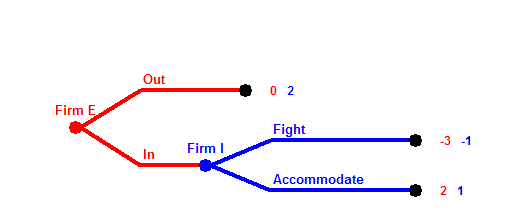
\includegraphics[width=0.8\linewidth]{Predation_game}
\end{center}
\begin{itemize}{\small
\item There are two pure strategy Nash equilibria in the game.
\item One equilibrium is (Out, Fight if Firm E chooses ``In'')
\item The other equilibrium is (In, Accommodate if Firm E chooses ``In'')}
\end{itemize}
\end{frame}



\stepcounter{slidenum}
\begin{frame}[fragile]
\frametitle{Example \arabic{examplecount}}
\framesubtitle{Market entry (\arabic{slidenum})}
The Nash equilibria can be checked from the strategic-form representation of the game:
\begin{center}
\begin{game}{2}{2}[Firm~E][Firm~I]
 \> Fight if \textbf{E} plays ``In'' \> Accommodate if \textbf{E} plays ``In'' \\
Out \> $ 0,2 $ \> $ 0,2 $ \\
In \> $ -3,-1 $ \> $ 2,1 $
\end{game}
\end{center}\bigskip
{\small
\textbf{Question:} Isn't (Out, Accommodate if Firm E chooses ``In'') a Nash equilibrium as well? \bigskip \pause 

\begin{itemize}
\item However, one of the two pure strategy Nash equilibria, the equilibrium (Out, Fight if Firm E chooses ``In''), isn't very plausible.
\item This is because once Firm E has decided to enter, it is not optimal for Firm I to fight.
\item Firm E can figure that out, so in real life it is likely to enter.
\end{itemize}}
\end{frame}


\stepcounter{slidenum}
\begin{frame}[fragile]
\frametitle{Example \arabic{examplecount}}
\framesubtitle{Market entry (\arabic{slidenum})}
\begin{itemize}\itemsep1em
\item Effectively, what happens in this game is that the incumbent makes an empty threat and the concept of Nash equilibrium implies that the entrant will take it seriously.
\item By virtue of the sequential nature of the game, under Nash equilibrium Player I can declare that it will do anything in the unreached branch of the game and its statement will affect the decision of the other player.
\item This suggests that we may want to strengthen our criteria for optimality of play by taking on board the implications of the sequential structure of decision-making in a dynamic game.
\end{itemize}
\end{frame}



\begin{frame}[fragile]
\frametitle{The principle of sequential rationality}
\framesubtitle{}
\begin{itemize}\itemsep1em
\item The previous considerations suggest that equilibrium strategies should specify behaviour that is optimal not only in general but also in a ``piecewise'' manner, from any point in the game onward.
\item This requirement is known as the \emph{principle of sequential rationality}.
\item Operationally, the principle of sequential rationality for games of perfect information is implemented by a procedure known as \emph{backward induction}.
\end{itemize}
\end{frame}



\begin{frame}[fragile]
\frametitle{Backward induction and subgames}
\framesubtitle{}
\begin{itemize}\itemsep1em
\item Roughly, backward induction means that we solve that game starting from the end and reconstructing optimal behaviour by moving toward the initial node of the game tree.
\item In order to do that we need a unit for which to consider optimality when going backward.
\item A natural candidate for such a unit is a subset of the game tree that itself constitutes a game when taken in isolation.
\item Such a subset is called a \emph{subgame}.
\end{itemize}
\end{frame}


\begin{frame}[fragile]
\frametitle{The backward induction procedure}
The backward induction procedure can be summarised as follows:
\begin{enumerate}\itemsep1em
\item \label{itm:1} Find the minimal subgames containing the terminal nodes and compute their Nash equilibria.
\item Replace the subgames with the equilibrium payoffs associated with a Nash equilibrium and produce a reduced game. (In case of multiple Nash equilibria the procedure is repeated).
\item Go to step \ref{itm:1} and repeat the procedure for the new, reduced game. Continue until you have included the subgame containing the initial node.
\end{enumerate}\bigskip

The collections of moves obtained via the backward induction procedure define strategies that are consistent with the principle of sequential rationality.
\end{frame}



\begin{frame}[fragile]
\frametitle{Subgame perfect Nash equilibria}
\begin{itemize}\itemsep1em
\item A profile of strategies that induces a Nash equilibrium for every subgame of a given extensive-form game is called a \emph{subgame perfect Nash equilibrium}.
\item Applying the backward induction procedure to an extensive-form game of perfect information by construction produces a subgame perfect Nash equilibrium.
\item Every finite game of perfect information has a pure strategy subgame perfect Nash equilibrium. If no player has the same payoffs at any two terminal nodes, then there is a unique subgame perfect Nash equilibrium.
\end{itemize}
\end{frame}



\stepcounter{examplecount}\setcounter{slidenum}{1}
\begin{frame}[fragile]
\frametitle{Example \arabic{examplecount}}
\framesubtitle{Backward induction in action (\arabic{slidenum})}
Consider the following game:
\begin{center}
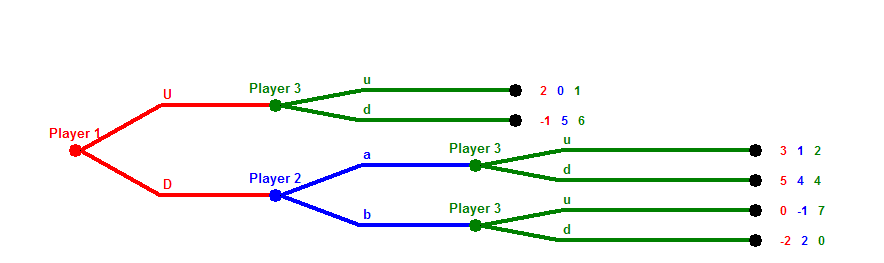
\includegraphics[width=0.9\linewidth]{Backward_induction_1}
\end{center}\bigskip

\begin{itemize}{\small
\item The three subgames containing the terminal nodes all belong to Player 3 and are shown in green.
\item Solving them (from top to bottom in the figure) reveals that Player 3 will play respectively $ d $, $ d $ and $ u $.
\item We replace the subgames with the respective payoffs.}
\end{itemize}
\end{frame}


\stepcounter{slidenum}
\begin{frame}[fragile]
\frametitle{Example \arabic{examplecount}}
\framesubtitle{Backward induction in action (\arabic{slidenum})}
The resulting reduced game is:
\begin{center}
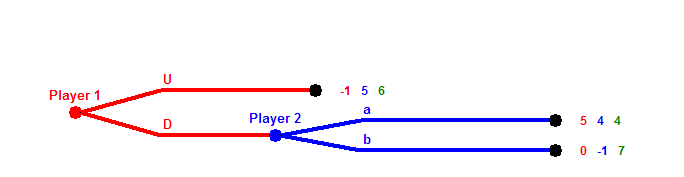
\includegraphics[width=0.9\linewidth]{Backward_induction_2}
\end{center}\bigskip

\begin{itemize}{\small
\item The next level subgame belongs to Player 2 and is shown in blue.
\item The equilibrium in this subgame is $ a $.
\item We repeat the reduction procedure and replace the subgame with the resulting payoff.}
\end{itemize}
\end{frame}


\stepcounter{slidenum}
\begin{frame}[fragile]
\frametitle{Example \arabic{examplecount}}
\framesubtitle{Backward induction in action (\arabic{slidenum})}
The final reduced game is:
\begin{center}
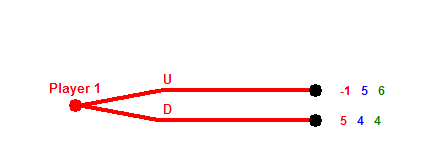
\includegraphics[width=0.65\linewidth]{Backward_induction_3}
\end{center}\bigskip

\begin{itemize}{\small
\item It is optimal for Player 1 to choose $ D $ in this subgame.
\item As this is the reduced game containing the initial node, this ends the backward induction procedure.
\item The final set of payoffs is $ (5,4,4) $ and it will be obtained by the sequence of moves $ D \rightarrow a \rightarrow d $.}
\end{itemize}
\end{frame}


\stepcounter{slidenum}
\begin{frame}[fragile]
\frametitle{Example \arabic{examplecount}}
\framesubtitle{Backward induction in action (\arabic{slidenum})}
\begin{itemize}\itemsep1em
\item Notice, however, that the strategies leading to the above sequence of moves are more complicated. 
\item These strategies are:
	\begin{itemize}\itemsep1em
	\item \textbf{Player 1:} Play $ D $.
	\item \textbf{Player 2:} Play $ a $ if Player 1 plays $ D $.
	\item \textbf{Player 3:} Play $ d $ if Player 1 plays $ U $. \newline Play $ d $ if Player 1 plays $ D $ and Player $ 2 $ plays $ a $. \newline Play $ u $ if Player 1 plays $ D $ and Player $ 2 $ plays $ b $.
	\end{itemize}
\item The above strategy profile is a subgame perfect Nash equilibrium for the game.
\end{itemize}
\end{frame}

\begin{frame}[fragile]
\frametitle{Exercise on the game from Example \arabic{examplecount}}
\framesubtitle{}
\begin{enumerate}\itemsep1em
\item Input the game in Gambit.
\item Try to compute a Nash equilibrium for the game. Instruct Gambit to compute all Nash equilibria. 
\item What happens when you explore dominance?
\end{enumerate}
\end{frame}



%%%%%%%%%%%%%%%%%%%%%%%%%%%%%
\section{Useful topics not covered in this lecture}
%%%%%%%%%%%%%%%%%%%%%%%%%%%%%

\begin{frame}[fragile]
\frametitle{General remarks}
\framesubtitle{}
\begin{itemize}\itemsep1em
\item Game theory is a vast and proliferating subject. It is impossible to give a comprehensive overview of its current state.
\item However, certain topics feature regularly in game theory courses and we can at least mention some of them for future reference.
\item Even in this case we can only give an incomplete and highly stylized list that is necessarily subjective.
\item Take a look at the sources in the References section for more information and additional ideas.
\end{itemize}
\end{frame}

\begin{frame}[fragile]
\frametitle{Equilibrium refinements}
\begin{itemize}\itemsep1em
\item Nash equilibrium is a very useful concept but it is not devoid of limitations.
\item Outcomes that are legitimate Nash equilibria may be deemed unrealistic if assessed on common plausibility grounds, as the example with the market entry game shows.
\item These considerations have spawned a branch of game theory focusing on selecting specific equilibria based on additional criteria.
\item This is known as \emph{equilibrium refinement}.
\item There exist various equilibrium concepts refining the Nash equilibrium. (Subgame perfection is one example.) They are useful in different situations and there isn't one universally established refinement dominating the game-theoretic literature.
\end{itemize}
\end{frame}

\begin{frame}[fragile]
\frametitle{Incomplete information}
\begin{itemize}\itemsep1em
\item We mentioned games of incomplete information without actually studying them.
\item This is not for lack of importance: many problems of practical relevance can be modelled as games of incomplete information.
\item Examples of these include:
	\begin{itemize}\itemsep1em
	\item Market entry with no information on the incumbents' costs
	\item Trade negotiations
	\item Auctions
	\end{itemize}
\end{itemize}
\end{frame}


\begin{frame}[fragile]
\frametitle{Repeated games}
\begin{itemize}\itemsep1em
\item In certain contexts one game may be played over and over by the same players.
\item This situation is known as a \emph{repeated game}.
\item A repeated game enriches the potential for strategic interaction and allows strategies that would not be used by rational players in a one-shot game.
\item As an example, in a repeated Prisoner's Dilemma cooperation can emerge as a viable strategy, unlike the case of the one-shot game.
\end{itemize}
\end{frame}

\begin{frame}[fragile]\setcounter{slidenum}{1}
\frametitle{Differential games (\arabic{slidenum})}
\begin{itemize}\itemsep1em
\item Recall that a continuous-time optimal control problem is a dynamic optimization problem in which the constraints are given by differential equations (the state equations). 
\item A simple version of a state equation may read \[ \dot{x}(t) = f(x(t),u(t)). \]
\item Now suppose that there are two planning entities, each having their own objective functional and controls. The latter are denoted respectively by $ u_1(t) $ and $ u_2(t) $.
\item Suppose further that the state equation is \[ \dot{x}(t) = f(x(t),u_1(t),u_2(t)), \]
i.e. it features both controls.
\end{itemize}
\end{frame}

\begin{frame}[fragile]\stepcounter{slidenum}
\frametitle{Differential games (\arabic{slidenum})}
\begin{itemize}\itemsep1em
\item Thus, the two entities are now interdependent, since they have a common state equation with partial control over it by virtue of having their own control.
\item Such a situation is called a \emph{differential game}. 
\item Differential games have various applications, e.g. in marketing, public finance, optimal resource exploitation and even military warfare.
\end{itemize}
\end{frame}

\setcounter{slidenum}{1}
\begin{frame}[fragile]
\frametitle{Evolutionary games (\arabic{slidenum})}
\begin{itemize}\itemsep1em
\item Imagine a situation in which a game is played repeatedly in a population of individuals, who are matched randomly against one another in every round of play.
\item There are different subsets of the population favouring different (fixed) strategies. This may be the result of rational deliberation or simply an innate preference.
\item As the game progresses, groups employing more successful strategies grow in size, while groups using less successful strategies shrink.
\item This is similar to a Darwinian survival-of-the-fittest process where evolution eliminates species that are unable to cope in their habitat.
\item Such games are called \emph{evolutionary games}.
\end{itemize}
\end{frame}

\begin{frame}[fragile]\stepcounter{slidenum}
\frametitle{Evolutionary games (\arabic{slidenum})}
\begin{itemize}\itemsep1em
\item Evolutionary games are important because they open the possibility that rational behaviour may emerge in the limit as the result of an adaptive process akin to learning.
\item In particular, some Nash equilibria can materialize as stable outcomes in appropriately defined evolutionary games.
\item This is more flexible and realistic compared to the assumption that individuals are perfectly rational from the start, which may imply almost superhuman reasoning powers of the participating players.
\end{itemize}
\end{frame}


\begin{frame}[fragile]
\frametitle{References}
\begin{itemize}\itemsep1em
	\item Mas-Colell, Whinston, Green. \emph{Microeconomic Theory}. 1995. Part 2.
	\item Osborne, Rubinstein. \emph{A Course in Game Theory}. 1994.
	\item Machler, Solan, Zamir. \emph{Game Theory}. 2013.
	\item Fudenberg, Tirole. \emph{Game Theory}. 1991.
	\item Ge\c ckil, Anderson. \emph{Applied Game Theory and Strategic Behavior}. 2010.
\end{itemize}
\end{frame}

\end{document}